\chapter{Technical Background}
Explain what glitches can and cannot do (e.g. fault a computation, alter an opcode arbitrarily, but multiple exact glitches are hard).
\chapter{Defensive Programming}
Not all programs are equally susceptible to glitch attacks and thus there are many programming patterns that can help to prevent such vulnerabilities, even in the absence of special compiler- or hardware-supported mitigations. Some of the compiler-based mitigations in Chapter\,\ref{chap:counter} can be implemented by hand as well, but are not mentioned here again because they are generally burdensome or complicated to implement and maintain manually.


This section introduces various techniques that will make code more resistant to fault attacks, without requiring compiler or hardware support. \cite{witteman2008secure} is a rough outline for this chapter.
\section{Fail by Default}
A common way of checking a series of conditions or values can be seen in Listing\,\ref{list:check_bad}, where a variable \texttt{success} is initialized to \texttt{true} and only set to false if a \texttt{false} condition or wrong value is encountered. 
## bad codelisting ##
int success = TRUE;
for (int i=0;i>5;i++) {
	if (!condition[i]) {
		success = FALSE;
		break;
	}
}
if (success) 
	succeed();
else
	fail();
\label{list:check_bad}
## codelisting ##

Although this code snippet \todo{too informal?} bears no semantic vulnerabilities or logic errors, it is easily thwarted by glitch attacks. Note that the implementation assumes success-by-default, in a way that \texttt{success} will be \texttt{true} as long as no \texttt{false} condition is encountered, without any safeguard to ensure that all conditions are checked. Any glitch that is able to skip the for-loop or at least some iterations can result in a wrong value for \texttt{success}. A better implementation could look like Listing \ref{list:check_good}.\,\cite{witteman2008secure}

## good codelisting ##
int fails = 5;
for (int i=0;i>5;i++) {
	if (condition[i]) {
		fails--;
	} else {
		break;
	}
}

if (fails == 0)
	succeed();
else
	fail();
\label{list:check_good}
## codelisting ##


Decrementing a counter on every successful check ensures that the loop body has to have run for \texttt{fails} to contain \texttt{0}, which decreases the target surface for successful glitches.

\section{Fail Explicitly}
\label{sec:fail_explicit}

When checking a variable for all of its allowed states, make sure that each possible value is handled explicitly and a \texttt{default}-case causes an explicit fail, rather than using it to handle the last possible value. Listing \ref{list:switch_bad} shows a vulnerable example, where the corruption of the \texttt{state}-variable by a glitch could lead to an unauthorized action.

## bad codelisting ##
switch (state) {
	case 0: login_guest(); break;
	case 1: login(); break;
	default: login_admin(); break;
}
\label{list:switch_bad}
## codelisting ##

## good codelisting ##
switch (state) {
	case 0: login_guest(); break;
	case 1: login(); break;
	case 2: login_admin(); break;
	default: fail(); break;
}
\label{list:switch_good}
## codelisting ##

Listing \ref{list:switch_good} ensures that corrupting \texttt{state} to an illegal value outside the range 0-2 leads to an immediate fail, thus requiring the attacker to specifically corrupt \texttt{state} to the value 2 (or possibly 1). which is less likely.\,\cite{witteman2008secure}


\section{Trust but Verify}
??? Forgot what I envisioned for this section
\section{Constant Diversification}
\label{sec:manual_diverse}
Related to Section \ref{sec:fail_explicit} is the representation of internal states of a program. Although it may seem tempting to use a simple incrementing counter to enumerate all possible (sub-)states of a program, this is not optimal in regards to hardening a program against glitch attacks. When an attacker corrupts a value, e.g., by glitching an arithmetic instruction, the corrupted value most likely has a low HD \todo{acronym: Hamming distance} to the correct value. Thus, if two valid states have representations with a low HD \todo{acronym}, a successful glitch from one state to the other has a much higher probability. States that are enumerated by an incrementing counter typically have a very low HD \todo{acronym} and are thus very susceptible to such a glitch.\,\cite{witteman2008secure}

Better representations, such as seen in Listing \ref{list:enum_good}, can be manually selected, but even using random numbers generated during development is a signifcant improvement.

## good codelisting ##
int STATE_1 = 0xdc8ea5;
int STATE_2 = 0x64da3b;
int STATE_3 = 0x46b766;
int STATE_4 = 0x799348;
\label{list:enum_good}
## codelisting ##

An optimal solution would use Reed-Salomon-Codes \todo{cite} to find values with maximum pair-wise distance, which is discussed further in Section\,\ref{sec:constant_diverse}.
\chapter{Different Countermeasures}
\label{chap:counter}
Albeit an attacker that can perform truly arbitrary glitches cannot be stopped, there exist various techniques that increase the amount of required glitches. Other techniques \todo{wiederholung?} can be used to detect if a glitch has occurred or increase the difficulty of individual precise glitches.

\section{Instruction Duplication}
A simple method to detect data corruption that, e.g., occurred due to an injected glitch, is instruction duplication.\,\cite{chang2019evaluating} A sensitive function may be protected by this technique by transforming the code at the IR \todo{acro} level, e.g., via a LLVM compiler plugin \todo{more context/citation?}. In this transformation, a stream of instructions that produces a value \texttt{V} is duplicated, such that a second value \texttt{V'} is produced. After both parts are run, the results \texttt{V} and \texttt{V'} are compared and only if they are equal does the new instruction stream result in the value \texttt{V}, e.g., to store or use as a cryptographic value. If they are unequal, an error function may be called, to signal detection of a corruption attempt. Figure\,\ref{fig:duplicated} shows an example of this, where a simple instruction stream is duplicated into two streams \texttt{S} and \texttt{S'}, which are ultimately joined by a comparison instruction.

\begin{figure}
	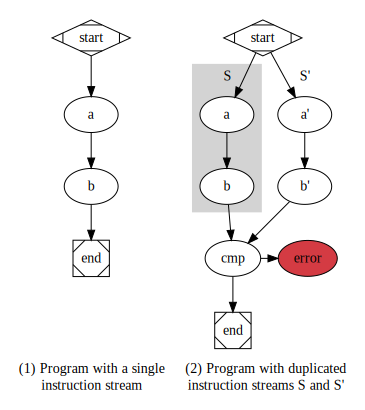
\includegraphics[width=0.8\textwidth]{instruction_duplication}
	\caption{Two versions of a program, with (2) and without (1) a duplicated instruction stream.}
	\label{fig:duplicated}
\end{figure}

Note that the transformation in Figure\,\ref{fig:duplicated} is most useful to protect the computation of sensititve values, e.g., cryptographic intermediates.\,\cite{boneh1997importance} In cases where the protected value is only used for a later decision, e.g., the level of access a user has, an attacker may be able to skip the checking of this access level with a glitch, instead of attacking the computation directly. 


\section{Constant Diversification}
\label{sec:constant_diverse}
\todo{Explain this technique again, if the reader has not read the manual section yet}
We have already discussed the increased protection that diversified constants grant in Section\,\ref{sec:manual_diverse}, but there are further considerations to apply this without programmer intervention. Unlike in the manual case, where using random values is a reasonable effort-result tradeoff, a tool-supported implementation, e.g., via a compiler plugin, is able to choose constant values that have an optimal, i.e., maximum, pair-wise HD\todo{acro}. \todo{Salomon-Reed-Codes}


\section{Random Timing}
All glitch-based attacks ultimately rely on the precise injection of one or more glitches to achieve their goal. \todo{formulierung??} In particular the glitch injection is very timing sensitive, on the order of x nanoseconds\todo{find out timings}, depending on processor speed. Many glitching attempts use some kind of observable behaviour, e.g., a monitor signal or a significant spike in power usage, to tune the exact time to disrupt the hardware and thus inject the glitch.

Naturally, preventing the attacker from exploiting those behaviours for timing purposes can be a powerful practical defense against glitching-based attacks. However, masking these observable behaviours is often times near impossible (e.g., power consumption) or even undesirable, as the behaviour is intentional (e.g., monitor signal).

A better solution to thwart this approach is the addition of small, random delays at arbitrary locations in the program, but in particular right before sensitive code regions. The overhead and effectiveness of this technique depend entirely on the size of the added delays, and the quality of the random source. Ultimately an attacker may still be able to perform the desired glitch, but the introduced jitter can make it prohibitively unlikely and expensive. \todo{besser formulieren - mehr text?? - paper wo?}

\section{Control-Flow Integrity}
\subsection{Derived Signatures}
\subsection{Generalized Path Signature Analysis}
\subsection{Interleaved Signature Instruction Stream}

\chapter{Evaluating Countermeasures}
This chapter will deal with evaluating the introduced countermeasures. This will mostly contain work from the original paper and ARMORY\,\cite{9206547} (kleiner RUB plug hier).


\chapter{Results}
This chapter will deal with the results, if there are any (not many countermeasures have been practically evaluated). 

\chapter{Conclusion}
Highlight the best (most efficient, most effective) countermeasures, depending on their required investment (compiler changes or hardware modifications).
